% Options for packages loaded elsewhere
\PassOptionsToPackage{unicode}{hyperref}
\PassOptionsToPackage{hyphens}{url}
%
\documentclass[
  english,
  man,floatsintext]{apa6}
\usepackage{amsmath,amssymb}
\usepackage{lmodern}
\usepackage{ifxetex,ifluatex}
\ifnum 0\ifxetex 1\fi\ifluatex 1\fi=0 % if pdftex
  \usepackage[T1]{fontenc}
  \usepackage[utf8]{inputenc}
  \usepackage{textcomp} % provide euro and other symbols
\else % if luatex or xetex
  \usepackage{unicode-math}
  \defaultfontfeatures{Scale=MatchLowercase}
  \defaultfontfeatures[\rmfamily]{Ligatures=TeX,Scale=1}
\fi
% Use upquote if available, for straight quotes in verbatim environments
\IfFileExists{upquote.sty}{\usepackage{upquote}}{}
\IfFileExists{microtype.sty}{% use microtype if available
  \usepackage[]{microtype}
  \UseMicrotypeSet[protrusion]{basicmath} % disable protrusion for tt fonts
}{}
\makeatletter
\@ifundefined{KOMAClassName}{% if non-KOMA class
  \IfFileExists{parskip.sty}{%
    \usepackage{parskip}
  }{% else
    \setlength{\parindent}{0pt}
    \setlength{\parskip}{6pt plus 2pt minus 1pt}}
}{% if KOMA class
  \KOMAoptions{parskip=half}}
\makeatother
\usepackage{xcolor}
\IfFileExists{xurl.sty}{\usepackage{xurl}}{} % add URL line breaks if available
\IfFileExists{bookmark.sty}{\usepackage{bookmark}}{\usepackage{hyperref}}
\hypersetup{
  pdftitle={Preferring Politeness: Young children's implicit comprehension of linguistic politeness},
  pdfauthor={Hannah E. Marshall1, Rondeline M. Williams1, \& Michael C. Frank1},
  pdflang={en-EN},
  pdfkeywords={politeness, language acquisition, pragmatic development, online experiment},
  hidelinks,
  pdfcreator={LaTeX via pandoc}}
\urlstyle{same} % disable monospaced font for URLs
\usepackage{graphicx}
\makeatletter
\def\maxwidth{\ifdim\Gin@nat@width>\linewidth\linewidth\else\Gin@nat@width\fi}
\def\maxheight{\ifdim\Gin@nat@height>\textheight\textheight\else\Gin@nat@height\fi}
\makeatother
% Scale images if necessary, so that they will not overflow the page
% margins by default, and it is still possible to overwrite the defaults
% using explicit options in \includegraphics[width, height, ...]{}
\setkeys{Gin}{width=\maxwidth,height=\maxheight,keepaspectratio}
% Set default figure placement to htbp
\makeatletter
\def\fps@figure{htbp}
\makeatother
\setlength{\emergencystretch}{3em} % prevent overfull lines
\providecommand{\tightlist}{%
  \setlength{\itemsep}{0pt}\setlength{\parskip}{0pt}}
\setcounter{secnumdepth}{-\maxdimen} % remove section numbering
% Make \paragraph and \subparagraph free-standing
\ifx\paragraph\undefined\else
  \let\oldparagraph\paragraph
  \renewcommand{\paragraph}[1]{\oldparagraph{#1}\mbox{}}
\fi
\ifx\subparagraph\undefined\else
  \let\oldsubparagraph\subparagraph
  \renewcommand{\subparagraph}[1]{\oldsubparagraph{#1}\mbox{}}
\fi
% Manuscript styling
\usepackage{upgreek}
\captionsetup{font=singlespacing,justification=justified}

% Table formatting
\usepackage{longtable}
\usepackage{lscape}
% \usepackage[counterclockwise]{rotating}   % Landscape page setup for large tables
\usepackage{multirow}		% Table styling
\usepackage{tabularx}		% Control Column width
\usepackage[flushleft]{threeparttable}	% Allows for three part tables with a specified notes section
\usepackage{threeparttablex}            % Lets threeparttable work with longtable

% Create new environments so endfloat can handle them
% \newenvironment{ltable}
%   {\begin{landscape}\begin{center}\begin{threeparttable}}
%   {\end{threeparttable}\end{center}\end{landscape}}
\newenvironment{lltable}{\begin{landscape}\begin{center}\begin{ThreePartTable}}{\end{ThreePartTable}\end{center}\end{landscape}}

% Enables adjusting longtable caption width to table width
% Solution found at http://golatex.de/longtable-mit-caption-so-breit-wie-die-tabelle-t15767.html
\makeatletter
\newcommand\LastLTentrywidth{1em}
\newlength\longtablewidth
\setlength{\longtablewidth}{1in}
\newcommand{\getlongtablewidth}{\begingroup \ifcsname LT@\roman{LT@tables}\endcsname \global\longtablewidth=0pt \renewcommand{\LT@entry}[2]{\global\advance\longtablewidth by ##2\relax\gdef\LastLTentrywidth{##2}}\@nameuse{LT@\roman{LT@tables}} \fi \endgroup}

% \setlength{\parindent}{0.5in}
% \setlength{\parskip}{0pt plus 0pt minus 0pt}

% \usepackage{etoolbox}
\makeatletter
\patchcmd{\HyOrg@maketitle}
  {\section{\normalfont\normalsize\abstractname}}
  {\section*{\normalfont\normalsize\abstractname}}
  {}{\typeout{Failed to patch abstract.}}
\patchcmd{\HyOrg@maketitle}
  {\section{\protect\normalfont{\@title}}}
  {\section*{\protect\normalfont{\@title}}}
  {}{\typeout{Failed to patch title.}}
\makeatother
\shorttitle{Preferring Politeness}
\keywords{politeness, language acquisition, pragmatic development, online experiment\newline\indent Word count: X}
\usepackage{lineno}

\linenumbers
\usepackage{csquotes}
\ifxetex
  % Load polyglossia as late as possible: uses bidi with RTL langages (e.g. Hebrew, Arabic)
  \usepackage{polyglossia}
  \setmainlanguage[]{english}
\else
  \usepackage[main=english]{babel}
% get rid of language-specific shorthands (see #6817):
\let\LanguageShortHands\languageshorthands
\def\languageshorthands#1{}
\fi
\ifluatex
  \usepackage{selnolig}  % disable illegal ligatures
\fi
\newlength{\cslhangindent}
\setlength{\cslhangindent}{1.5em}
\newlength{\csllabelwidth}
\setlength{\csllabelwidth}{3em}
\newenvironment{CSLReferences}[2] % #1 hanging-ident, #2 entry spacing
 {% don't indent paragraphs
  \setlength{\parindent}{0pt}
  % turn on hanging indent if param 1 is 1
  \ifodd #1 \everypar{\setlength{\hangindent}{\cslhangindent}}\ignorespaces\fi
  % set entry spacing
  \ifnum #2 > 0
  \setlength{\parskip}{#2\baselineskip}
  \fi
 }%
 {}
\usepackage{calc}
\newcommand{\CSLBlock}[1]{#1\hfill\break}
\newcommand{\CSLLeftMargin}[1]{\parbox[t]{\csllabelwidth}{#1}}
\newcommand{\CSLRightInline}[1]{\parbox[t]{\linewidth - \csllabelwidth}{#1}\break}
\newcommand{\CSLIndent}[1]{\hspace{\cslhangindent}#1}

\title{Preferring Politeness: Young children's implicit comprehension of linguistic politeness}
\author{Hannah E. Marshall\textsuperscript{1}, Rondeline M. Williams\textsuperscript{1}, \& Michael C. Frank\textsuperscript{1}}
\date{}


\authornote{

All code, data, figures, cited papers, and pre-planned analyses are publicly available at \url{https://github.com/HannahEveMarshall/preferring_politeness}. The current study, including all analyses, was registered on OSF prior to data collection: \url{https://osf.io/dz8vp}.

}

\affiliation{\vspace{0.5cm}\textsuperscript{1} Stanford University}

\abstract{
Adults routinely demonstrate social sensitivity by utilizing polite speech. But when do children begin to comprehend linguistic politeness? Existing literature indicates that basic comprehension of polite speech presents early in development: by 3 years, children accurately judge whether a speaker is more polite, ruder, nicer, or meaner than another based on the speaker's use of polite speech (Yoon \& Frank, 2019). By 4 years, children reliably opt for play partners who use politeness markers; however, previous studies have not observed reliable preference for a polite speaker in children younger than 4 years, potentially due to experimental task demands. This project proposes a less challenging paradigm (adapted from similar shape-preference paradigms, i.e.~Hamlin, Wynn, \& Bloom, 2007; Thomas \& Sarnecka, 2019), which may detect preference for a polite speaker in children younger than 4 years. In addition to informing our understanding of children's sociolinguistic development, this study aims to demonstrate the effectiveness of a simpler paradigm for future studies of linguistic politeness in young children.
}



\begin{document}
\maketitle

To engage in successful social interactions, an individual must demonstrate social sensitivity. The same individual must assess the social sensitivity of others to determine the desirability of their social partners. The capacity to evaluate individuals on the basis of their social interactions is universal and unlearned (Haidt \& Joseph, 2004; Hamlin, Wynn, \& Bloom, 2007; Hauser, 2006; Pinker, 2003). Even preverbal infants develop social preferences based on individuals' behavior toward others (Hamlin, Wynn, \& Bloom, 2007). Through development, humans learn to routinely demonstrate and assess social sensitivity by employing and interpreting linguistic politeness in speech.

Linguistic politeness can be defined as a set of social behaviors, expressed verbally, which maintain, enhance, or challenge interpersonal relations (Vergis \& Pell, 2020). It is a form of social etiquette, which regulates the choice of communicative forms, structures, and set phrases a person uses (Ryabova, 2015). Being polite is considered a part of adult pragmatic competence, and the rules include, Don't impose, Give options, and Make the addressee feel good (Lakoff, 1973).

When speaking politely, individuals typically do not behave rationally in accordance with Gricean Maxims: in fact, polite speech violates theories of effective communication by typically being inefficient and under-informative (Grice, 1975; Yoon, Tessler, Goodman, \& Frank, 2020). Then why speaking politely? A utility-theoretic approach to speech acts suggest that polite speech emerges from a tradeoff between three competing goals of communication: to convey information (informational utility), to be kind (prosocial utility), and to present oneself in a good light (self-presentational utility) (Yoon, Tessler, Goodman, \& Frank, 2020).

\hypertarget{composing-a-polite-utterance}{%
\subsection{Composing a Polite Utterance}\label{composing-a-polite-utterance}}

Speaking with an appropriate degree of politeness comes intuitively to most adults; however, formulating an adequately polite utterance is a fairly complex process. Ervin-Tripp (1977) asserted that two factors affect the production and comprehension of polite register: knowledge of the linguistic form of polite requests and knowledge of pragmatic request rules within a given social and situational context (1977). Figure 1 expands on these two factors by illustrating what an adult with normative socio-pragmatic competence typically considers before producing a polite utterance.

\begin{figure}
\centering
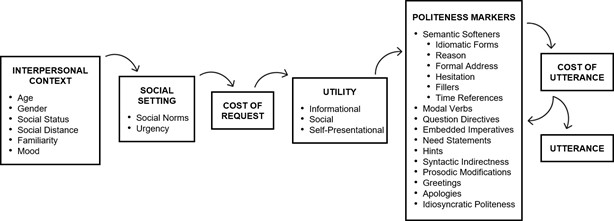
\includegraphics{C:/Users/Hannah/Desktop/preferring_politeness/figures/diagrams/contextual_considerations.jpg}
\caption{Considerations when selecting a polite utterance.}
\end{figure}

In selecting a polite utterance, an individual must first consider the interpersonal context of their interaction. To be appropriately polite, the individual must vary their level and form of politeness depending on the difference between their own and their interlocutor's ages, genders, and social statuses. For example, it may be more appropriate for a younger person to speak more politely to an older person than vice versa, and it may be more appropriate for a male to speak more politely to a female than to another male. Similarly, a person of high social status may speak with a level of politeness that is indicative of their sophistication but also does not compromise their face.

After considering the interpersonal context of their interaction, a person must consider the degree of politeness which is appropriate for the unique social setting. For instance, a sense of urgency makes it more appropriate to opt for the imperative (and less polite) phrase ``Call an ambulance, now,'' as opposed to asking, ``Ms.~Smith, when you have a moment, would you mind calling an ambulance, please?''

After considering the interpersonal context and social setting of their interaction, a person must consider the cost of their request and decide how informative they want to be, how kind they want to be, and how informative and kind they want to present themselves as. In doing so, the person must determine their ideal, balanced weightings of the informational, social, and self- presentational utilities of their utterance.

Then, the individual must consult their internal inventory of politeness markers and selectively compose an utterance which is appropriate for the social setting, interpersonal context, and content of their request, as well as satisfies their desired utilities.

Finally, the person must weigh the cost of their utterance. If the cost is reasonable, then the person would make the utterance, and if the utterance is too costly, the person would return to their inventory of polite language to compose a less costly utterance.

At each step in this process, the speaker must not only judge the literal meaning of their utterance; they must also predict the listener's interpretation to ensure that their utterance effectively communicates the intended message. Thus, the production of polite speech can be understood through a Rational Speech Act framework, characterized by recursive reasoning.

According to this framework, the speaker chooses to produce a polite utterance based on their prediction of how a listener would interpret it, and the listener being reasoned about interprets the utterance by reasoning about the speaker's prediction, and so on (Yoon, Tessler, Goodman, \& Frank, 2020).

\hypertarget{acquisition-of-politeness}{%
\subsection{Acquisition of Politeness}\label{acquisition-of-politeness}}

Being suitably polite involves masterfully combining an understanding of social and contextual factors with an inventory of linguistic forms. The complexity of this ability brings into question when and how humans being to acquire polite speech.

Production of polite speech begins early in development: At two years old, children modify their requests to adjust politeness (Bates \& Silvern, 1977), and at two and a half years old, children produce ``please'' (Read \& Cherry, 1978). By three years old, children are able to vary their utterances based on whether they are instructed to ``tell'' versus ``ask'' an addressee to give them a puzzle piece (Bock \& Hornsby, 1981). By three years old, children also possess several politeness formulas in their repertoires and use them spontaneously and appropriately quite frequently in their home context (Eisenberg, 1982).

Evidence from studies on children's understanding of politeness indicates that that children understand the implications of polite speech early on: By three years old, English- speaking preschool children can correctly identify whether a person is nicer, meaner, more polite, or less polite than another speaker, based on which speaker includes politeness markers such as ``please'' in their requests (Yoon \& Frank, 2019). By four years old, English-speaking preschool children tend to choose polite speakers as play partners over non-polite speakers and understand that polite speakers are more likely to have their requests granted (Yoon \& Frank, 2019). However, previous studies have not observed reliable preference for a polite speaker in children younger than four years, potentially due to experimental task demands (busy stimuli, excessive auditory input, high attention demands, etc.).

\hypertarget{the-current-study}{%
\subsection{The Current Study}\label{the-current-study}}

This study proposes a less challenging task based on existing shape-preference paradigms (Hamlin, Wynn, \& Bloom, 2007; Thomas \& Sarnecka, 2019), which could detect preference for a polite speaker in children younger than four years. We tested two-year-old, three-year-old, and four-year-old children's implicit understanding of linguistic politeness by assessing their preference for a polite speaker over an impolite speaker.

\hypertarget{hypotheses}{%
\subsubsection{Hypotheses}\label{hypotheses}}

\begin{enumerate}
\def\labelenumi{\arabic{enumi}.}
\item
  Considering our less challenging task, we predicted that two-year-old, three-year-old, and four-year-old children would indicate preference for a polite speaker over an impolite speaker (i.e.~the proportion of children in each age category who indicated preference for a polite speaker would differ from chance).
\item
  Considering evidence for graded comprehension of politeness in young children (Yoon \& Frank, 2019), we predicted that children would indicate preference for a polite speaker over an impolite speaker more reliably (i.e.~with a stronger effect) with increasing age.
\end{enumerate}

\hypertarget{methods}{%
\section{Methods}\label{methods}}

\hypertarget{participants}{%
\subsection{Participants}\label{participants}}

Participants included two-year old (n = 20), three-year-old (n = 20), and four-year-old (n = 20) children living in the U.S. at the time of data collection. Participants were recruited through the Department of Psychology at Stanford University through Facebook advertisements, Children Helping Science (an online recruitment platform for developmental research), and direct outreach to preschools and day cares in the Bay Area.

We selected our sample size based on a Bayesian power analysis conducted in R. Our lowest-power tests were by-age-category Bayesian binomial tests. To detect an effect in which 80\% of children indicate preference for a polite speaker with 80\% power and a 95\% credible interval, we had to run 15 participants in each age category (45 total). We ran 60 participants to compensate for exclusions and missing data. A second power analysis showed that with 60 participants, across age categories, we could detect an effect in which 70\% of children indicate preference for a polite speaker with 80\% power and a 95\% credible interval.

We excluded a child from the study if:

\begin{enumerate}
\def\labelenumi{\arabic{enumi}.}
\item
  The child was known to have any cognitive, auditory, or visual impairment, and the impairment was reported by the parent.
\item
  The child was known to have any neurodevelopmental disorder that significantly affects cognitive processing or social cognition, such as down syndrome or autism spectrum disorder, and the disorder was reported by the parent. Attention deficit disorder and attention deficit hyperactivity disorder were only grounds for exclusion if the child was unable to adequately complete test trials due to inattention or restlessness as per criterion 6.
\item
  The child did not hear English ``all of the time'' or ``most of the time'' as indicated by the parent upon registration.
\item
  A non-participant (e.g.~the child's parent or sibling) interjected or interfered by pointing at the screen at any time during the experiment, audibly commenting, or providing a response to either dependent variable measure (DV).
\item
  The child failed to provide a response to DV1 after four prompts.
\item
  The child was looking away from the screen for at least 25\% of the animation.
\item
  The child was looking away from the screen during either speaker utterance.
\item
  The parent rated the video or audio quality below a 3 out of 5.
\end{enumerate}

Based on these criteria, we excluded five children: two 2-year-old children and three 3-year-old children.

\hypertarget{stimuli}{%
\subsection{Stimuli}\label{stimuli}}

The animation began with a (secondary) familiarization phase in which a shape (the speaker) entered from the left of the screen, spotted two cookies on the opposite side of the screen, gasped excitedly, approached the cookies, ate one cookie, and celebrated by jumping up and down. The purpose of this phase was to inform the participant that the speaker's goal was to eat a cookie.

A testing phase followed in which the speaker entered from the left of the screen and stopped in front of another shape (the listener), who was standing in the way of the cookies. In the polite condition, the speaker said, ``I am so hungry! May I have a cookie please?'' In the impolite condition, the speaker said, ``I am so hungry! Give me a cookie now.'' Regardless of condition, the listener moved out of the speaker's way. The speaker gasped excitedly, crossed in front of the listener, approached the cookies, ate one cookie, and celebrated by jumping up and down.

Utterances used in the animation were prerecorded. Intonation was naturalistic and did not include exaggerated ``polite'' or ``impolite'' prosody. Utterances were cleaned using Audacity (an audio editing and recording software) and RMS was standardized across conditions using Praat (a phonetics software).

The background consisted of a solid, green block and solid, blue block depicting grass and sky. The listener was always a blue circle. The polite and impolite speakers consisted of either a red triangle and yellow square or a yellow triangle and red square. The triangle and square were the same height and width. The shape of the speaker (triangle/square), color of the shape (red/yellow), and order of the conditions (first/second) were counterbalanced across trials.

\hypertarget{randomization}{%
\subsection{Randomization}\label{randomization}}

A generic list randomizer was used to assign the first 16 participants in each age category to one of 16 uniquely counterbalanced animations (without repeats). The same generic list randomizer was used to assign the remaining 4 participants in each age category to one of the 16 animations (without repeats).

\hypertarget{procedure}{%
\subsection{Procedure}\label{procedure}}

Children completed the study on their family's home or personal computers with an experimenter online via Zoom (a videotelephony software). A parent had to provide either written consent via email or verbal consent prior to testing. The attending parent was notified that they or their child may stop participation at any time. Testing sessions were recorded with parental consent. Each session began by testing audio quality and calibrating the participant's screen settings.

The experimenter began with a warm-up activity to build rapport with the child. The experimenter played a short ``I-Spy'' game with the child, during which a black and white dog emerged from behind a pile of leaves, then a brown squirrel emerged from the same pile. To avoid inducing side bias, the animals were front-facing and centered, and the pile of leaves was symmetrical.

Next, in the primary familiarization, the experimenter introduced the child to a green pentagon, which had eyes and a mouth to indicate animacy. The experimenter then showed the child what the character looks like when it ``feels very sad'' (downturned mouth), ``feels normal'' (flat-line mouth), and ``feels very happy'' (upturned, open mouth). The purpose of this primary phase was to introduce shapes as animate characters and to accustom the participant to facial expressions that would be seen in the upcoming animation.

After the primary familiarization phase, the animation was played. Each participant saw both the polite condition and the impolite condition as detailed above. The experimenter was not blind to condition but bared a blank expression and looked down while the animation was playing. At the end of the animation, the caregiver attending to the child was asked to close their eyes before the child's preference and reasoning were assessed.

We measured preference between a polite speaker and an impolite speaker by presenting a forced-choice in which the speakers appear on opposite sides of the screen (counterbalanced) and the participant was asked, ``Which friend do you want to play with?'' (DV1, our key dependent variable measure).

Pointing, reaching, and verbal answers were coded equivalently as indication of preference. If a child did not answer, the child was prompted three more times with analogous wording. If the child did not provide an answer after four prompts, the session was concluded. If the child provided an answer, the child was then asked, ``Why do you want to play with that friend?'' (DV2, a supplementary dependent variable measure). If the child did not provide an answer, the child was prompted twice more.

Including screen setup and debriefing, each session took approximately 10 to 15 minutes to complete. Children nor parents were financially compensated for participating in the study.

\hypertarget{coding-and-inferences}{%
\subsection{Coding and Inferences}\label{coding-and-inferences}}

Age category was coded to consist of three levels:

\begin{itemize}
\item
  2-year-olds (2 years, 0 months \(\leqslant\) x \textless{} 3 years, 0 months)
\item
  3-year-olds (3 years, 0 months \(\leqslant\) x \textless{} 4 years, 0 months)
\item
  4-year-olds (4 years, 0 months \(\leqslant\) x \textless{} 5 years, 0 months)
\end{itemize}

DV1 was dummy coded with preference for the polite speaker as 1 and preference for the impolite speaker as 0. DV2 was coded to include:

\begin{itemize}
\item
  No reasoning: no explanation after a third prompt (e.g., silence, shrugging, or ``I don't know'').
\item
  Superficial reasoning: any explanation regarding elements besides speaker utterance (e.g., ``I like him,'' ``He's red,'' ``Triangles are my favorite'').
\item
  Logical reasoning: any explanation that refers to speaker utterance and is consistent with the animation (e.g., describing the polite speaker as ``nice'' or ``polite'').
\item
  Other reasoning: any explanation that does not fall under classifications 1 -- 3 (e.g., an intelligible response).
\end{itemize}

Our study utilized pairwise deletion: If a child did not complete DV2, their DV1 data was still included in analyses. We included all data-based outliers in our analyses.

Two-tailed tests were used for each of our analyses. We made inferences based on credible intervals, using a 95\% credible interval criterion for success.

\hypertarget{results}{%
\section{Results}\label{results}}

After data collection was complete, we will run a Bayesian binomial test from the BayesianFirstAid package in R to assess whether the proportion of children in our sample who indicated preference for a polite speaker differed from chance.

We assessed whether the proportion of children in our sample who indicated preference for a polite speaker differed from chance using a Bayesian binomial test. We 58\% of our entire sample indicated preference for a polite speaker.

A logistic regression predicting speaker preference based on age showed a slightly positive--but not substantial--overall effect of age: Every 12-month increase in age predicted an increase of .1 in the probability that a child will indicate preference for a polite speaker.

Our data showed much more variation than was captured by our logistic regression (Figure 2). To capture this variation, we faceted out data by age category (two-year-old, three-year-old, and four-year-old children), and we assessed whether the proportion of children in each age category who indicated preference for a polite speaker differed from chance using additional Bayesian binomial tests. 65\% of two-year-old children, 36\% of three-year-old children, and 69\% of four-year-old children indicated preference for a polite speaker.

\begin{figure}
\centering
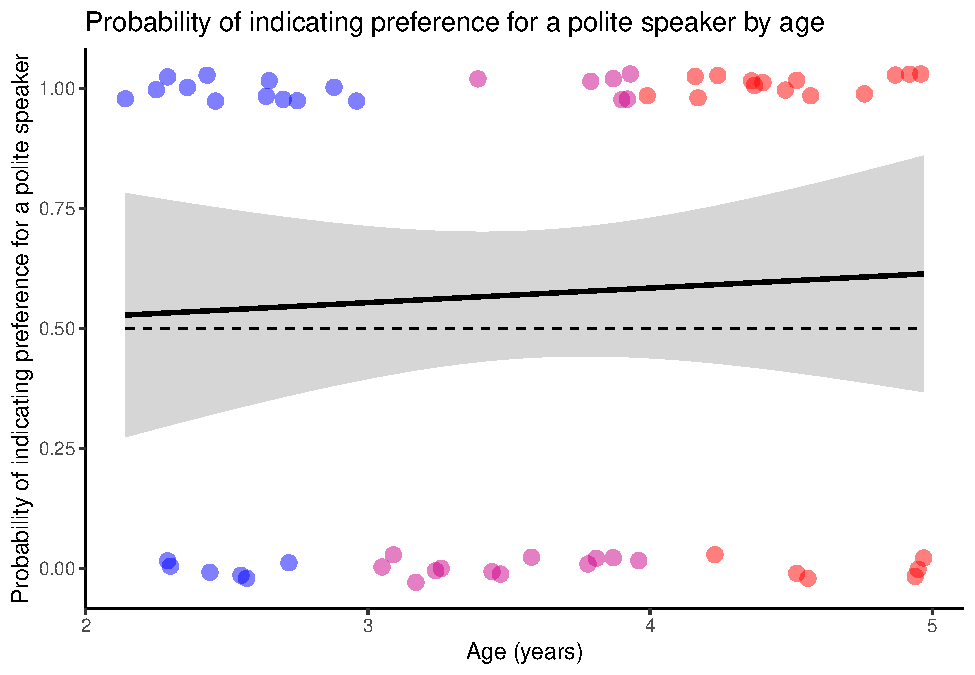
\includegraphics{writeup_files/figure-latex/unnamed-chunk-1-1.pdf}
\caption{\label{fig:unnamed-chunk-1}Each point represents an individual observation. Points have been jittered slightly (by .03 vertically) for readability. Black line represents a logistic regression.}
\end{figure}

\begin{figure}
\centering
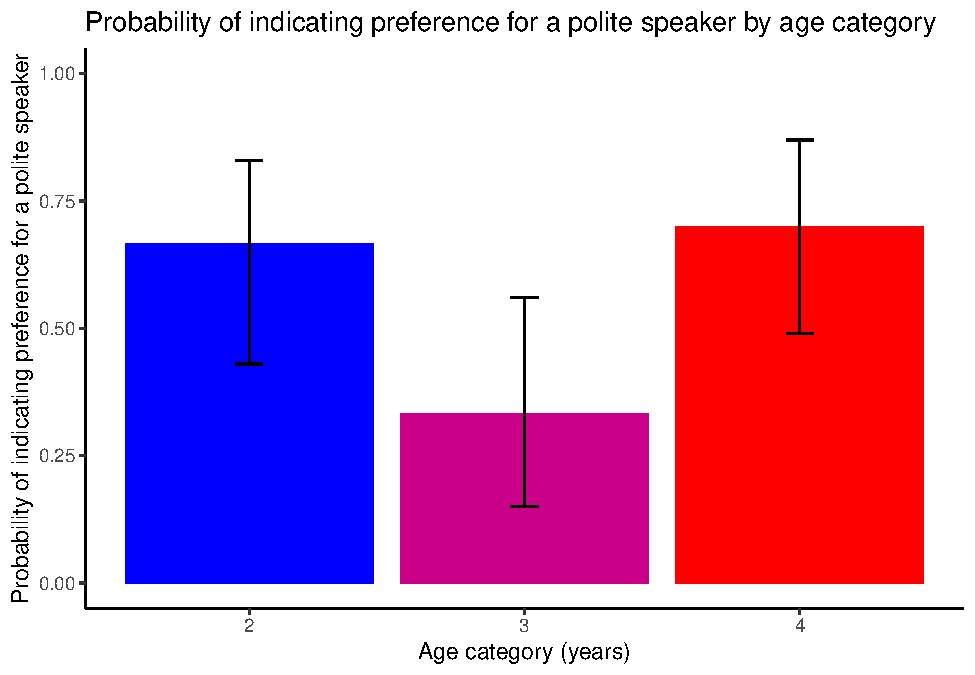
\includegraphics{writeup_files/figure-latex/unnamed-chunk-2-1.pdf}
\caption{\label{fig:unnamed-chunk-2}Each bar illustrates the mean response of participants in each age category, which is representative of the probability of indicating preference for a polite speaker. Error bars represent 95\% credible intervals based on Bayesian binomial tests.}
\end{figure}

\hypertarget{discussion}{%
\section{Discussion}\label{discussion}}

\begin{enumerate}
\def\labelenumi{\arabic{enumi}.}
\item
  Replicated prior research where four-year-old children reliably indicated preference for a polite speaker, but three-year-old children did not (Yoon).
\item
  But showed that two-year-olds can also do this!
\item
  Performance of two-year-old children is comparable to the performance of four-year-olld children, indicating that there is not a substantial developmental ``improvement'' between two and four years: All the cognitive capacities that goes into identifying polite language, forming an opinion about the speaker, and indicating a preference based on that is present at 2 years old.
\item
  Three-year-old children performed much differently than expected, showing a slight preference for the impolite speaker.

  \begin{itemize}
  \item
    Could be that 3-year-olds are just performing at chance. At this age, children start preschool, things like shape, color, object-referent language become salient, and things like social evaluation may be lost in the background.
    - By 4 years, children have developed a plethora of vocabulary and social evaluation, once again, become pertinent to assessing, engaging with, and relating to the people and world around them.
  \item
    Or could be that children may actually be preferring the impolite speaker.
    - There is vast and string evidence that young children prefer--and choose-- toys which function and characters who behave unexpectedly (\ldots; \ldots). At two, children may recognize polite language as prosocial, and therefore prefer it; but, at three, children might be more interested in exploring the social world and thus, pick the character whose utterance is the least expected.
    - A handful of the children giggled after the impolite speaker made its utterance. Some even credited their choice to the fact that the speaker was ``funny'' or ``silly.'' Anecdotally, young children are much less upset by other's words. If this is what the children are picking up on, they may be choosing the speaker that says something entertaining.
  \end{itemize}
\end{enumerate}

\hypertarget{limitations}{%
\subsection{Limitations}\label{limitations}}

\begin{itemize}
\item
  Context in stimuli is actually quite foreign to many children. From a very young age, if a child asks for something nicely, they get the thing, and if they ask for something rudely, they will be corrected by an adult (e.g., ``What do you say?'' or ``What's the magic word?''). In our animation, both the polite character and impolite character's wishes were granted. This may have exacerbated any effect that was due to the unexpectedness of the impolite speaker.
\item
  Because politeness is so broad, this study and specific scenario really only gets at children's preference for a polite speaker in a very small portion of polite phenomena
\end{itemize}

\hypertarget{future-directions}{%
\subsection{Future directions}\label{future-directions}}

\begin{itemize}
\tightlist
\item
  Restate findings
\item
  Implications
\end{itemize}

In future:
- Replicate results
- Study a broader range of scenarios involving politeness
- Study other aspects of politeness

\hypertarget{references}{%
\section{References}\label{references}}

\begingroup
\setlength{\parindent}{-0.5in}
\setlength{\leftskip}{0.5in}

\hypertarget{refs}{}
\begin{CSLReferences}{1}{0}
\leavevmode\hypertarget{ref-bates1977}{}%
Bates, E., \& Silvern, L. (1977). Social adjustment and politeness in preschoolers. \emph{Journal of Communication}.

\leavevmode\hypertarget{ref-bock1981}{}%
Bock, J. K., \& Hornsby, M. E. (1981). The development of directives: How children ask and tell. \emph{Journal of Child Language}, \emph{8}(1), 151--163.

\leavevmode\hypertarget{ref-eisenberg1982}{}%
Eisenberg, A. R. (1982). Understanding components of a situation: Spontaneous use of politeness routines by mexicano 2-year-olds.

\leavevmode\hypertarget{ref-ervintripp1977}{}%
Ervin-Tripp, S. (1977). Wait for me, roller skate! In \emph{Child discourse} (pp. 165--188). Elsevier.

\leavevmode\hypertarget{ref-grice1975}{}%
Grice, H. P. (1975). Logic and conversation. In \emph{Speech acts} (pp. 41--58). Brill.

\leavevmode\hypertarget{ref-haidt2004}{}%
Haidt, J., \& Joseph, C. (2004). Intuitive ethics: How innately prepared intuitions generate culturally variable virtues. \emph{Daedalus}, \emph{133}(4), 55--66.

\leavevmode\hypertarget{ref-hamlin2007}{}%
Hamlin, J. K., Wynn, K., \& Bloom, P. (2007). Social evaluation by preverbal infants. \emph{Nature}, \emph{450}(7169), 557--559.

\leavevmode\hypertarget{ref-hauser2006}{}%
Hauser, M. (2006). \emph{Moral minds: How nature designed our universal sense of right and wrong.} Ecco/HarperCollins Publishers.

\leavevmode\hypertarget{ref-lakoff1973}{}%
Lakoff, R. (1973). The logic of politeness; or, minding your p's and q's. In \emph{Ninth regional meeting of the chicago linguistic society} (Vol. 8, pp. 292--305). 292J305. Chicago: Chicago Linguistic Society.

\leavevmode\hypertarget{ref-pinker2003}{}%
Pinker, S. (2003). Language as an adaptation to the cognitive niche. \emph{Studies in the Evolution of Language}, \emph{3}, 16--37.

\leavevmode\hypertarget{ref-read1978}{}%
Read, B. K., \& Cherry, L. J. (1978). Preschool children's production of directive forms. \emph{Discourse Processes}, \emph{1}(3), 233--245.

\leavevmode\hypertarget{ref-ryabova2015}{}%
Ryabova, M. (2015). Politeness strategy in everyday communication. \emph{Procedia-Social and Behavioral Sciences}, \emph{206}, 90--95.

\leavevmode\hypertarget{ref-thomas2019}{}%
Thomas, A. J., \& Sarnecka, B. W. (2019). Infants choose those who defer in conflicts. \emph{Current Biology}, \emph{29}(13), 2183--2189.

\leavevmode\hypertarget{ref-vergis2020}{}%
Vergis, N., \& Pell, M. D. (2020). Factors in the perception of speaker politeness: The effect of linguistic structure, imposition and prosody. \emph{Journal of Politeness Research}, \emph{16}(1), 45--84.

\leavevmode\hypertarget{ref-yoon2019}{}%
Yoon, E. J., \& Frank, M. C. (2019). Preschool children's understanding of polite requests. In \emph{CogSci} (pp. 3179--3185).

\leavevmode\hypertarget{ref-yoon2020}{}%
Yoon, E. J., Tessler, M. H., Goodman, N. D., \& Frank, M. C. (2020). Polite speech emerges from competing social goals. \emph{Open Mind}, \emph{4}, 71--87.

\end{CSLReferences}

\endgroup


\end{document}
